\documentclass{beamer}

\usetheme{Frankfurt}

\title{Workshop 11 -- Problem Solving}
\author{COMP20005 Engineering Computation}
\institute{The University of Melbourne}

\begin{document}

\renewcommand{\tt}[1]{\texttt{#1}}

\begin{frame}
    \titlepage
\end{frame}

\begin{frame}{Contact Info}
    \begin{itemize}
        \item Matt Signorini
        \item Email: \tt{msignorini@unimelb.edu.au}
        \item Also LMS discussion forum for help
        \item My workshop solutions available at \url{https://github.com/pkill-9/comp20005-workshops/}
    \end{itemize}
\end{frame}

\begin{frame}{Today's Workshop}
    \begin{block}{Agenda}
        By the end of this class, you should:
        \begin{itemize}
            \item Be able to identify an appropriate problem solving
                strategy for a particular problem.
        \end{itemize}
    \end{block}
\end{frame}

\section{Exercises}
\stepcounter{subsection}

\begin{frame}{9.7}
    Devise a mechanism for determining the set of adjacent elements in an
    array that has the largest sum.

    Note that this problem is trivial when the array contains entirely
    positive numbers; however when there are positive and negative numbers
    you must be able to decide which elements are part of the sum and
    which are not.

    Which of the problem solving techniques do you think might provide an
    algorithm to solve this problem?
\end{frame}


\section{Lab Exercises}
\stepcounter{subsection}

\begin{frame}{Exercises}
    \begin{block}{Lab Problems}
        \begin{itemize}
            \item[9.3] Program to deal cards for Poker.
            \item[9.11] Rocket flight simulation.
        \end{itemize}
    \end{block}
\end{frame}

\begin{frame}{9.11}
    For those who don't have the blue book\ldots
    \begin{figure}
        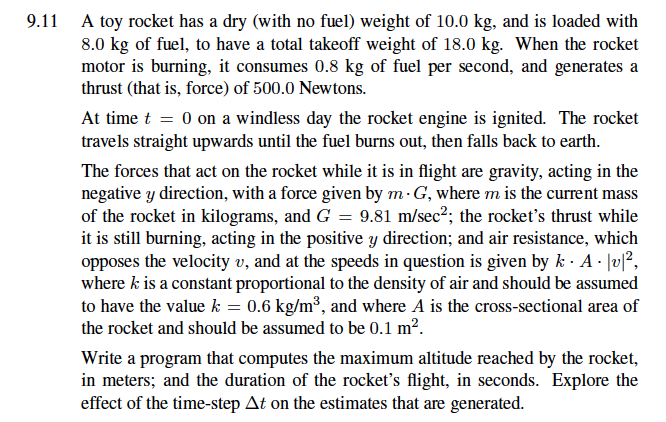
\includegraphics[width=10cm]{e09-11.png}
    \end{figure}
\end{frame}

%
%
% No ASCII art this week. No, this weeks easter egg is something far more
% valuable.
%
% Did you *really* think that I made those pretty pictures all by hand?
% Of course I didn't, that would be an enourmously labrious task. Instead,
% I used a shell script to run some programs that generate an ASCII art
% figure and quotation at random. You can do it too:
%
% LINUX INSTRUCTIONS (works on Ubuntu):
%
% 1. Install some packages
%
% sudo apt-get install cowsay
% sudo apt-get install fortune-mod
% sudo apt-get install fortunes
%
%
%
% 2. Running this shell script will generate random ASCII arts.
%
% =================
% #! /bin/bash
%
% # First, choose a character at random from all the possible figures that
% # cowsay can print.
% COWFILE = `ls /usr/share/cowsay/cows/ | sort -R | head -1`
%
% # Choose a random quote from these tech related topics. You can remove
% # the topics, then it will choose a quote from all topics.
% fortune perl computers debian linux linuxcookie education | cowsay -f ${COWFILE}
% =================
%
% You can also add the contents of this script to your .bashrc file, then
% every time you open up a terminal you will be greeted with a random (and
% often very funny) message of the day.
%
%
%
% WINDOWS INSTRUCTIONS:
%
% 1. Download linux image for the distribution of your choice (I
% reccommend Ubuntu, but it's up to you)
%
% 2. Install linux.
%
% 3. Proceed with linux instructions above.
%
% :)
%


\end{document}

% vim: ft=tex ts=4 sw=4 lbr et
